\chapter{Leçon 27: Am Schonggeschäft}

Dës Lektioun beschäftegt sech mat engem Dialog an engem Schonggeschäft. Mir léieren, wéi ee Schong keeft, wéi ee Froen iwwer d'Gréisst, de Präis an d'Qualitéit stellt, an typesch Ausdréck fir d'Lieder ze fleegen. Mir studéieren och d'Konjugatioun vum Verb \textbf{bäissen} an de Gebrauch vum Adjektiv \textbf{futti}, souwéi de wichtege sproochlechen Ënnerscheed tëscht de Partikelen \textbf{och}, \textbf{nach} an \textbf{och nach}. \textit{Cette leçon traite d'un dialogue dans un magasin de chaussures. Nous apprenons comment acheter des chaussures, comment poser des questions sur la pointure, le prix et la qualité, et des expressions typiques pour entretenir le cuir. Nous étudions également la conjugaison du verbe \textbf{bäissen} (mordre) et l'utilisation de l'adjectif \textbf{futti} (cassé / fatigué), ainsi que la différence linguistique importante entre les particules \textbf{och} (aussi), \textbf{nach} (encore) et \textbf{och nach} (en plus). / This lesson deals with a dialogue in a shoe shop. We learn how to buy shoes, ask questions about shoe size, price, and quality, and common expressions for caring for leather. We also study the conjugation of the verb \textbf{bäissen} (to bite) and the use of the adjective \textbf{futti} (broken / exhausted), as well as the important linguistic difference between the particles \textbf{och} (also), \textbf{nach} (still/another), and \textbf{och nach} (as well/in addition).}

\vspace{1em}

\section[Dialog: Am Schonggeschäft / Dialogue : Au magasin de chaussures / Dialogue: At the shoe shop]{Dialog: Am Schonggeschäft \\/ Dialogue : Au magasin de chaussures \\/ Dialogue: At the shoe shop}

Hei ass en typeschen Dialog tëscht dem Verkeefer an dem Client, mat de sproochleche Korrekturen aus eiser Lektioun: \\
\textit{Voici un dialogue typique entre le vendeur et le client, avec les corrections linguistiques de notre leçon : / Here is a typical dialogue between the shop assistant and the customer, featuring the linguistic corrections from our lesson:}

\vspace{1em}

\noindent\textbf{SCÈNE I -- De Client kënnt eran}

\noindent\textbf{1. Verkeefer: Moien, kann ech Iech hëllefen?}\\
\textit{Moien} (Bonjour / Hello), \textit{kann ech} (puis-je / can I) \textit{Iech hëllefen} (vous aider / help you)?\\
$\rightarrow$ Français : \textit{Bonjour, puis-je vous aider ?}\\
$\rightarrow$ English : \textit{Hello, can I help you?}\\[0.5em]

\noindent\textbf{2. Client: Moien, jo, ech sichen nei Schong.}\\
\textit{Moien} (Bonjour / Hello), \textit{jo} (oui / yes), \textit{ech sichen} (je cherche / I am looking for) \textit{nei Schong} (de nouvelles chaussures / new shoes).\\
$\rightarrow$ Français : \textit{Bonjour, oui, je cherche de nouvelles chaussures.}\\
$\rightarrow$ English : \textit{Hello, yes, I am looking for new shoes.}\\[0.5em]

\noindent\textbf{3. Verkeefer: Fir den Alldag oder éischter eppes Elegantes?}\\
\textit{Fir} (Pour / For) \textit{den Alldag} (le quotidien, tous les jours / everyday wear) \textit{oder} (ou / or) \textit{éischter} (plutôt / rather) \textit{eppes Elegantes} (quelque chose d'élégant / something elegant)?\\
$\rightarrow$ Français : \textit{Pour tous les jours ou plutôt quelque chose d'élégant ?}\\
$\rightarrow$ English : \textit{For everyday wear or rather something elegant?}\\[0.5em]

\noindent\textbf{4. Client: Fir d'éischt den Alldag, mee se sollen trotzdeem awer gutt ausgesinn.}\\
\textit{Fir d'éischt} (D'abord / First) \textit{den Alldag} (le quotidien / everyday wear), \textit{mee} (mais / but) \textit{se sollen} (elles doivent / they should) \textit{trotzdeem awer} (quand même / still) \textit{gutt ausgesinn} (avoir l'air bien, avoir du style / look good).\\
$\rightarrow$ Français : \textit{D'abord pour tous les jours, mais j'aimerais qu'elles soient quand même élégantes.}\\
$\rightarrow$ English : \textit{First for everyday wear, but they should still look good.}\\[0.5em]

\noindent\textbf{SCÈNE II -- De Verkeefer weist Modeller}

\noindent\textbf{5. Verkeefer: Hei hu mir e puer Modeller. Dës hei si ganz bequeem.}\\
\textit{Hei hu mir} (Voici, ici nous avons / Here we have) \textit{e puer Modeller} (quelques modèles / a few models). \textit{Dës hei} (Ceux-ci, celles-ci / These ones here) \textit{si ganz bequeem} (sont très confortables / are very comfortable).\\
$\rightarrow$ Français : \textit{Voici quelques modèles. Ceux-ci sont très confortables.}\\
$\rightarrow$ English : \textit{Here we have a few models. These ones here are very comfortable.}\\[0.5em]

\noindent\textbf{6. Client: Kann ech se probéieren?}\\
\textit{Kann ech} (Puis-je / Can I) \textit{se probéieren} (les essayer / try them on)?\\
$\rightarrow$ Français : \textit{Je peux les essayer ?}\\
$\rightarrow$ English : \textit{Can I try them on?}\\[0.5em]

\noindent\textbf{7. Verkeefer: Natierlech. Wéi eng Gréisst hutt Dir normalerweis?}\\
\textit{Natierlech} (Bien sûr / Of course). \textit{Wéi eng Gréisst} (Quelle pointure, quelle taille / What size) \textit{hutt Dir} (avez-vous / do you have) \textit{normalerweis} (d'habitude / normally)?\\
$\rightarrow$ Français : \textit{Bien sûr. Quelle pointure faites-vous d'habitude ?}\\
$\rightarrow$ English : \textit{Of course. What size do you normally wear?}\\[0.5em]

\noindent\textbf{8. Client: 43, mee heiansdo 44.}\\
\textit{43}, \textit{mee} (mais / but) \textit{heiansdo} (parfois / sometimes) \textit{44}.\\
$\rightarrow$ Français : \textit{43, mais parfois 44.}\\
$\rightarrow$ English : \textit{43, but sometimes 44.}\\[0.5em]

\noindent\textbf{9. Verkeefer: Ech bréngen Iech béid.}\\
\textit{Ech bréngen Iech} (Je vous apporte / I will bring you) \textit{béid} (les deux / both).\\
$\rightarrow$ Français : \textit{Je vous apporte les deux.}\\
$\rightarrow$ English : \textit{I will bring you both.}\\[0.5em]

\noindent\textbf{SCÈNE III -- De Client probéiert Schong un}

\noindent\textbf{10. Client: Déi éischt sinn e bësse knapp.}\\
\textit{Déi éischt} (Les premières / The first ones) \textit{sinn} (sont / are) \textit{e bësse knapp} (un peu serrées / a bit tight).\\
$\rightarrow$ Français : \textit{Les premières sont un peu serrées.}\\
$\rightarrow$ English : \textit{The first ones are a bit tight.}\\[0.5em]

\noindent\textbf{11. Verkeefer: Da probéiert déi aner. Déi sinn e bësse méi breet.}\\
\textit{Da probéiert} (Alors essayez / Then try) \textit{déi aner} (les autres / the others). \textit{Déi sinn} (Elles sont / They are) \textit{e bësse méi breet} (un peu plus larges / a bit wider).\\
$\rightarrow$ Français : \textit{Alors essayez les autres. Elles sont un peu plus larges.}\\
$\rightarrow$ English : \textit{Then try the others. They are a bit wider.}\\[0.5em]

\noindent\textbf{12. Client: Oh, déi si vill méi bequeem. Wéi déi vu virdrun.}\\
\textit{Oh}, \textit{déi si} (celles-ci sont / these are) \textit{vill méi bequeem} (beaucoup plus confortables / much more comfortable). \textit{Wéi déi vu virdrun} (Que celles d'avant / Like the ones before).\\
$\rightarrow$ Français : \textit{Oh, celles-ci sont beaucoup plus confortables. Que celles d'avant.}\\
$\rightarrow$ English : \textit{Oh, these are much more comfortable. Like the ones before.}\\[0.5em]

\noindent\textbf{13. Verkeefer: Gitt e puer Schrëtt, fir ze kucken ob se Iech passen.}\\
\textit{Gitt} (Faites / Take) \textit{e puer Schrëtt} (quelques pas / a few steps), \textit{fir ze kucken} (pour voir / to check) \textit{ob se Iech passen} (si elles vous vont, si elles vous conviennent / if they fit you).\\
$\rightarrow$ Français : \textit{Faites quelques pas pour voir si elles vous conviennent.}\\
$\rightarrow$ English : \textit{Take a few steps to see if they fit you.}\\[0.5em]

\noindent\textbf{14. Client: Jo, dat fillt sech gutt un.}\\
\textit{Jo} (Oui / Yes), \textit{dat fillt sech... un} (cela se sent / that feels) \textit{gutt} (bien / good).\\
$\rightarrow$ Français : \textit{Oui, c'est confortable.}\\
$\rightarrow$ English : \textit{Yes, that feels good.}\\[0.5em]

\noindent\textbf{SCÈNE IV -- Froen iwwer Qualitéit a Präis}

\noindent\textbf{15. Client: Wéi ass d'Qualitéit? Hale se laang?}\\
\textit{Wéi ass} (Comment est / How is) \textit{d'Qualitéit} (la qualité / the quality)? \textit{Hale se laang} (Durent-elles longtemps / Do they last long)?\\
$\rightarrow$ Français : \textit{Comment est la qualité ? Durent-elles longtemps ?}\\
$\rightarrow$ English : \textit{How is the quality? Do they last long?}\\[0.5em]

\noindent\textbf{16. Verkeefer: Jo, se sinn aus richtegem Lieder an hunn eng flexibel Suel.}\\
\textit{Jo} (Oui / Yes), \textit{se sinn} (elles sont / they are) \textit{aus richtegem Lieder} (en cuir véritable / made of real leather) \textit{an hunn} (et ont / and have) \textit{eng flexibel Suel} (une semelle flexible / a flexible sole).\\
$\rightarrow$ Français : \textit{Oui, elles sont en cuir véritable avec une semelle flexible.}\\
$\rightarrow$ English : \textit{Yes, they are made of real leather and have a flexible sole.}\\[0.5em]

\noindent\textbf{17. Client: A wéi vill kaschte se?}\\
\textit{A wéi vill} (Et combien / And how much) \textit{kaschte se} (coûtent-elles / do they cost)?\\
$\rightarrow$ Français : \textit{Et combien coûtent-elles ?}\\
$\rightarrow$ English : \textit{And how much do they cost?}\\[0.5em]

\noindent\textbf{18. Verkeefer: Dëse Modell kascht 89 Euro.}\\
\textit{Dëse Modell} (Ce modèle / This model) \textit{kascht} (coûte / costs) \textit{89 Euro}.\\
$\rightarrow$ Français : \textit{Ce modèle coûte 89 euros.}\\
$\rightarrow$ English : \textit{This model costs 89 euros.}\\[0.5em]

\noindent\textbf{19. Client: Dat ass raisonnabel.}\\
\textit{Dat ass} (C'est / That is) \textit{raisonnabel} (raisonnable / reasonable).\\
$\rightarrow$ Français : \textit{C'est raisonnable.}\\
$\rightarrow$ English : \textit{That is reasonable.}\\[0.5em]

\noindent\textbf{SCÈNE V -- Accessoiren a Berodung}

\noindent\textbf{20. Verkeefer: Wann Dir wëllt, hu mir och eng Crème fir d'Lieder ze fleegen.}\\
\textit{Wann Dir wëllt} (Si vous voulez / If you want), \textit{hu mir och} (nous avons aussi / we also have) \textit{eng Crème} (une crème / a cream) \textit{fir d'Lieder ze fleegen} (pour entretenir le cuir / to care for the leather).\\
$\rightarrow$ Français : \textit{Si vous voulez, nous avons aussi une crème pour entretenir le cuir.}\\
$\rightarrow$ English : \textit{If you want, we also have a cream to care for the leather.}\\[0.5em]

\noindent\textbf{21. Client: Ass dat néideg?}\\
\textit{Ass dat} (Est-ce / Is that) \textit{néideg} (nécessaire / necessary)?\\
$\rightarrow$ Français : \textit{Est-ce nécessaire ?}\\
$\rightarrow$ English : \textit{Is that necessary?}\\[0.5em]

\noindent\textbf{22. Verkeefer: Et hëlleft, datt d'Schong méi laang schéi bleiwen.}\\
\textit{Et hëlleft} (Cela aide / It helps), \textit{datt d'Schong} (que les chaussures / that the shoes) \textit{méi laang} (plus longtemps / longer) \textit{schéi bleiwen} (restent belles / stay beautiful).\\
$\rightarrow$ Français : \textit{Cela aide à garder les chaussures belles plus longtemps.}\\
$\rightarrow$ English : \textit{It helps the shoes stay beautiful longer.}\\[0.5em]

\noindent\textbf{23. Client: Da huelen ech déi och nach dobäi.}\\
\textit{Da huelen ech} (Alors je prends / Then I take) \textit{déi} (celle-là / that) \textit{och nach} (aussi en plus / as well) \textit{dobäi} (avec, en plus / in addition).\\
$\rightarrow$ Français : \textit{Alors je la prends aussi en plus.}\\
$\rightarrow$ English : \textit{Then I'll take that as well.}\\[0.5em]

\noindent\textbf{SCÈNE VI -- Bezuelen}

\noindent\textbf{24. Verkeefer: Also, d'Schong an d'Crème, dat mécht zesummen 99 Euro.}\\
\textit{Also} (Alors / So), \textit{d'Schong an d'Crème} (les chaussures et la crème / the shoes and the cream), \textit{dat mécht zesummen} (cela fait ensemble / that makes in total) \textit{99 Euro}.\\
$\rightarrow$ Français : \textit{Alors, les chaussures et la crème, cela fait 99 euros en tout.}\\
$\rightarrow$ English : \textit{So, the shoes and the cream, that makes 99 euros in total.}\\[0.5em]

\noindent\textbf{25. Client: Ech bezuele mat der Kaart.}\\
\textit{Ech bezuelen} (Je paie / I pay) \textit{mat der Kaart} (avec la carte / by card).\\
$\rightarrow$ Français : \textit{Je paie par carte.}\\
$\rightarrow$ English : \textit{I'll pay by card.}\\[0.5em]

\noindent\textbf{26. Verkeefer: Merci. Hei ass Är Rechnung.}\\
\textit{Merci} (Merci / Thank you). \textit{Hei ass} (Voici / Here is) \textit{Är Rechnung} (votre ticket, votre facture / your receipt).\\
$\rightarrow$ Français : \textit{Merci. Voici votre ticket.}\\
$\rightarrow$ English : \textit{Thank you. Here is your receipt.}\\[0.5em]

\noindent\textbf{SCÈNE VII -- Ofschloss}

\noindent\textbf{27. Client: Merci fir Är Hëllef, ech si ganz zefridden.}\\
\textit{Merci fir} (Merci pour / Thank you for) \textit{Är Hëllef} (votre aide / your help), \textit{ech si} (je suis / I am) \textit{ganz zefridden} (très satisfait / very satisfied).\\
$\rightarrow$ Français : \textit{Merci pour votre aide, je suis très satisfait.}\\
$\rightarrow$ English : \textit{Thank you for your help, I am very satisfied.}\\[0.5em]

\noindent\textbf{28. Verkeefer: Gär geschitt. Schéinen Dag nach a vill Freed mat de Schong.}\\
\textit{Gär geschitt} (Je vous en prie, de rien / My pleasure). \textit{Schéinen Dag nach} (Bonne journée encore / Have a nice day still) \textit{a} (et / and) \textit{vill Freed} (beaucoup de plaisir / much joy) \textit{mat de Schong} (avec les chaussures / with the shoes).\\
$\rightarrow$ Français : \textit{Je vous en prie. Bonne journée et profitez bien de vos chaussures.}\\
$\rightarrow$ English : \textit{My pleasure. Have a nice day and enjoy your shoes.}\\[0.5em]

\noindent\textbf{29. Client: Merci, Iech och.}\\
\textit{Merci} (Merci / Thank you), \textit{Iech och} (à vous aussi / to you too).\\
$\rightarrow$ Français : \textit{Merci, à vous aussi.}\\
$\rightarrow$ English : \textit{Thank you, you too.}\\[0.5em]

\vspace{1cm}

\section[D'Verben an hire Gebrauch / Verbes / Verbs]{D'Verben an hire Gebrauch \\/ Les verbes et leur utilisation \\/ Verbs and their usage}

An dëser Lektioun hu mir e puer wichteg Verben begéint. Hei sinn hir Konjugatiounen an hire Gebrauch: \\
\textit{Dans cette leçon, nous avons rencontré plusieurs verbes importants. Voici leurs conjugaisons et leur utilisation : / In this lesson, we encountered several important verbs. Here are their conjugations and usage:}

\subsection*{1. Bäissen}
D'Verb \textbf{bäissen} bedeit \textbf{mordre} (to bite):

\begin{tabular}{ll c l l}
    \toprule
    \textbf{Pronom} & \textbf{Lëtzebuergesch} & \textbf{} & \textbf{Français} & \textbf{English} \\
    \midrule
    ech & bäissen & $\rightarrow$ & Je mords & I bite \\
    du & bäiss & $\rightarrow$ & Tu mords & You bite \\
    hien / hatt / et & bäisst & $\rightarrow$ & Il / Elle / On mord & He / She / It bites \\
    \midrule
    mir & bäissen & $\rightarrow$ & Nous mordons & We bite \\
    dir & bäisst & $\rightarrow$ & Vous mordez & You bite \\
    si & bäissen & $\rightarrow$ & Ils / Elles mordent & They bite \\
    \bottomrule
\end{tabular}
\\[0.5em]
\textbf{Passé Composé:} Forméiert mat \textit{hunn} + \textbf{gebass} (z.B. \textit{Den Hond huet mech gebass} $\rightarrow$ Le chien m'a mordu / The dog bit me).

\vspace{0.5em}
\noindent\textbf{Sproochlechen Tipp (Active vs. Passive):}
\begin{itemize}
    \item \textbf{Du bäiss} (active): Tu mords / You bite.
    \item \textbf{Du bass gebass} (stative/passive): Tu es mordu / You are bitten (Forméiert mat \textit{sinn} + \textit{gebass}).
    \item Beispill vum Dialog: \textit{Ech si vun engem Schof gebass ginn.} (J'ai été mordu par un mouton. / I was bitten by a sheep.)
\end{itemize}

\subsection*{2. Futtigoen}
D'Verb \textbf{futtigoen} (separabelt Verb: \textit{geet futti}) bedeit \textbf{tomber en panne} oder \textbf{se casser} (to break, to break down):
\begin{itemize}
    \item \textit{Mäi Computer geet séier futti.} (Mon ordinateur tombe vite en panne. / My computer breaks down quickly.)
    \item \textit{Mäi Vëlo ass gëschter futtigaangen.} (Mon vélo est tombé en panne hier. / My bike broke down yesterday.)
\end{itemize}

\vspace{1cm}

\section[Grammaire an Ausdréck / Grammaire / Grammar]{Grammaire an Ausdréck \\/ Grammaire et Expressions \\/ Grammar and Expressions}

Hei sinn e puer wichteg sproochlech Reegelen an Ausdréck aus eiser Lektioun: \\
\textit{Voici quelques règles linguistiques et expressions importantes de notre leçon : / Here are some important linguistic rules and expressions from our lesson:}

\subsection*{1. Och, Nach, an Och nach}
Dës dräi Partikele gi ganz dacks am Lëtzebuergesche benotzt, mee hunn ënnerschiddlech Bedeitungen: \\
\textit{Ces trois particules sont très souvent utilisées en luxembourgeois, mais ont des significations différentes : / These three particles are very often used in Luxembourgish, but have different meanings:}

\begin{itemize}
    \item \textbf{och} (aussi / also, too):
    \textit{Ech ginn och mat.} \\
    $\rightarrow$ French: \textit{Je viens aussi.} \\
    $\rightarrow$ English: \textit{I am coming too.} \\
    \textit{Merci, Iech och!} \\
    $\rightarrow$ French: \textit{Merci, à vous aussi !} \\
    $\rightarrow$ English: \textit{Thank you, you too!}
    
    \item \textbf{nach} (encore, de plus / still, yet, another):
    \textit{Hien ass nach an der Vakanz.} \\
    $\rightarrow$ French: \textit{Il est encore en vacances.} \\
    $\rightarrow$ English: \textit{He is still on vacation.} \\
    \textit{Schéinen Dag nach!} \\
    $\rightarrow$ French: \textit{Bonne journée encore !} \\
    $\rightarrow$ English: \textit{Have a nice day still!}
    
    \item \textbf{och nach} (en plus, également / as well, in addition):
    \textit{Da huelen ech déi Crème och nach dobäi.} \\
    $\rightarrow$ French: \textit{Alors je prends aussi cette crème en plus.} \\
    $\rightarrow$ English: \textit{Then I will take that cream as well.}
    
    \item \textbf{Wichteg (Important):} D'Reiefolleg \textit{nach och} ass falsch an däerf net benotzt ginn. \\
    $\rightarrow$ French: \textit{L'ordre des mots "nach och" est incorrect et ne doit pas être utilisé.} \\
    $\rightarrow$ English: \textit{The word order "nach och" is incorrect and must not be used.}
\end{itemize}

\subsection*{2. Futti}
D'Adjektiv \textbf{futti} huet am Lëtzebuergeschen zwou Haaptbedeitungen: \\
\textit{L'adjectif \textbf{futti} a deux significations principales en luxembourgeois : / The adjective \textbf{futti} has two main meanings in Luxembourgish:}

\begin{itemize}
    \item \textbf{Cassé / Foutu} (broken, out of order): \\
    \textit{Mäi Schong ass futti.} \\
    $\rightarrow$ French: \textit{Ma chaussure est cassée.} \\
    $\rightarrow$ English: \textit{My shoe is broken.}
    
    \item \textbf{Épuisé / Crevé} (completely exhausted): \\
    \textit{Ech sinn total futti nom Lafen.} \\
    $\rightarrow$ French: \textit{Je suis complètement crevé après avoir couru.} \\
    $\rightarrow$ English: \textit{I am completely exhausted after running.}
\end{itemize}

\noindent\textbf{Den Ausdrock (L'expression / The expression): Ech sinn dätsch}
\begin{itemize}
    \item Den Ausdrock \textbf{dätsch sinn} gëtt ëmgangssproochlech benotzt fir ze soen datt ee komplett geschafft oder exténué ass: \\
    \textit{L'expression \textbf{dätsch sinn} est utilisée familièrement pour dire que l'on est sur les rotules ou épuisé : / The expression \textbf{dätsch sinn} is used colloquially to say that one is knackered or shattered:}
    \item Beispill: \textit{Nodeems d'Kanner de ganzen Dag am Park gespillt haten, ware si ganz dätsch.} \\
    $\rightarrow$ French: \textit{Après que les enfants ont joué toute la journée dans le parc, ils étaient sur les rotules (complètement épuisés).} \\
    $\rightarrow$ English: \textit{After the children had played all day in the park, they were completely knackered.}
\end{itemize}

\subsection*{3. E bëssen / E bësse}
Am Lëtzebuergesche gëtt den Ausdrock fir \textbf{un peu / a little / a bit} ëmmer mam onbestëmmten Artikel \textbf{e} gebraucht: \textbf{e bëssen} (oder \textbf{e bësse}). Ee kann net einfach "bëssen" oder "bësse" ouni den Artikel soen: \\
\textit{En luxembourgeois, l'expression pour \textbf{un peu} est toujours utilisée avec l'article indéfini \textbf{e} : \textbf{e bëssen} (ou \textbf{e bësse}). On ne peut pas dire simplement "bëssen" ou "bësse" sans l'article. / In Luxembourgish, the expression for \textbf{a little / a bit} is always used with the indefinite article \textbf{e}: \textbf{e bëssen} (or \textbf{e bësse}). One cannot simply say "bëssen" or "bësse" without the article.}

\begin{itemize}
    \item \textbf{e bëssen / e bësse} (un peu / a little, a bit):
    \textit{Ech huelen e bësse Cash mat.} \\
    $\rightarrow$ French: \textit{J'emporte un peu d'argent liquide.} \\
    $\rightarrow$ English: \textit{I take a bit of cash with me.}
    
    \item \textbf{Eifeler Regel mat "bëssen":}
    D'Wuert \textbf{e bëssen} verléiert säin `n` a gëtt zu \textbf{e bësse} virun engem Konsonant (ausser n, d, t, z, h): \\
    \textit{Le mot \textbf{e bëssen} perd son `n` et devient \textbf{e bësse} devant une consonne (sauf n, d, t, z, h). / The word \textbf{e bëssen} drops its `n` and becomes \textbf{e bësse} before a consonant (except n, d, t, z, h).}
    \begin{itemize}
        \item \textit{e bësse knapp} (knapp fänkt mat `k` un $\rightarrow$ `n` fält ewech / knapp commence par `k` $\rightarrow$ le `n` tombe / knapp starts with `k` $\rightarrow$ `n` is dropped).
        \item \textit{e bësse méi breet} (méi fänkt mat `m` un $\rightarrow$ `n` fält ewech / méi commence par `m` $\rightarrow$ le `n` tombe / méi starts with `m` $\rightarrow$ `n` is dropped).
        \item \textit{e bëssen Angscht} (Angscht fänkt mat engem Vokal un $\rightarrow$ `n` bleift / Angscht commence par une voyelle $\rightarrow$ le `n` reste / Angscht starts with a vowel $\rightarrow$ `n` is kept).
    \end{itemize}
    
    \item \textbf{Gebrauch mat Verben:}
    Well deen Ausdrock ëmmer mam Artikel \textbf{e} gebraucht gëtt, gesäit dat viregt Verb eng Vokal (`e`). Dofir behält dat viregt Verb (wéi \textit{sinn}) säin `nn`: \\
    \textit{Comme cette expression est toujours précédée de l'article \textbf{e}, le verbe précédent rencontre une voyelle (`e`). Ainsi, le verbe précédent (comme \textit{sinn}) conserve son `nn`. / Because this expression is always preceded by the article \textbf{e}, the preceding verb encounters a vowel (`e`). Therefore, the preceding verb (such as \textit{sinn}) retains its `nn`.}
    \begin{itemize}
        \item \textit{Déi éischt} \textbf{sinn} \textit{e bësse knapp.} (richteg / correct)
        \item \textit{Déi éischt} \textbf{si} \textit{bësse knapp.} (falsch / incorrect -- den Artikel \textbf{e} feelt, an d'Eifeler Regel ass verletzt / l'article \textbf{e} manque et la règle d'Eifel est violée / the article \textbf{e} is missing and the Eifeler rule is violated)
    \end{itemize}
\end{itemize}

\subsection*{4. Eifeler Regel am Dialog}
Kuckt de Sproochgebrauch an de Sätz: \\
\textit{Observez l'usage de la langue dans ces phrases : / Observe the language usage in these sentences:}

\begin{itemize}
    \item \textit{Déi éischt} \textbf{sinn} \textit{e bësse knapp.} \\
    $\rightarrow$ \textit{Virun engem Vokal `e` gëtt de `nn` am Verb `sinn` beibehalen : `sinn`. / Devant une voyelle `e`, le `nn` du verbe `sinn` est conservé : `sinn`. / Before a vowel `e`, the `nn` in the verb `sinn` is retained: `sinn`.} \\
    $\rightarrow$ Français : \textit{Les premières sont un peu serrées.} \\
    $\rightarrow$ English : \textit{The first ones are a bit tight.}
    
    \item \textit{Déi} \textbf{sinn} \textit{e bësse méi breet.} \\
    $\rightarrow$ \textit{Virun engem Vokal `e` gëtt de `nn` beibehalen : `sinn`. / Devant une voyelle `e`, le `nn` est conservé : `sinn`. / Before a vowel `e`, the `nn` is retained: `sinn`.} \\
    $\rightarrow$ Français : \textit{Elles sont un peu plus larges.} \\
    $\rightarrow$ English : \textit{They are a bit wider.}
    
    \item \textit{Ech} \textbf{si} \textit{ganz zefridden.} \\
    $\rightarrow$ \textit{Virun engem Konsonant `g` gëtt de `nn` ewechgelooss : `si`. / Devant une consonne `g`, le `nn` est omis : `si`. / Before a consonant `g`, the `nn` is dropped: `si`.} \\
    $\rightarrow$ Français : \textit{Je suis très satisfait.} \\
    $\rightarrow$ English : \textit{I am very satisfied.}
\end{itemize}

\vspace{1.5cm}
\color{geminiBlue}\hrule height 1.5pt \vspace{0.5em}\color{black}
\section[Vokabulär: Neit Wierderbuch]{Vokabulär: Neit Wierderbuch \\/ Nouveau Vocabulaire Illustré \\/ New Illustrated Vocabulary}

\begin{itemize}
    \item \textbf{de Schong} (Pl.: d'Schong) $\rightarrow$ la chaussure (the shoe)
    \item \textbf{d'Suel} (Pl.: d'Suelen) $\rightarrow$ la semelle (the sole)
    \item \textbf{de Verkeefer} (Pl.: de Verkeefer) $\rightarrow$ le vendeur (the shop assistant, male)
    \item \textbf{d'Rechnung} (Pl.: d'Rechnungen) $\rightarrow$ la facture, le ticket (the receipt, invoice)
    \item \textbf{d'Schonggeschäft} (Pl.: d'Schonggeschäfter) $\rightarrow$ le magasin de chaussures (the shoe shop)
    \item \textbf{d'Lieder} (kee Pluriel) $\rightarrow$ le cuir (the leather)
    \item \textbf{futti} (adj.) $\rightarrow$ cassé, foutu / crevé (broken, out of order / exhausted)
    \item \textbf{dätsch} (adj.) $\rightarrow$ épuisé, sur les rotules (knackered, shattered)
\end{itemize}

\vspace{1em}

\begin{center}
    \begin{minipage}[t]{0.48\textwidth}
        \centering
        \textbf{E Schong}
        \vspace{0.5em}
        \framebox{\parbox{0.9\linewidth}{\centering
            \vspace{0.5cm}
            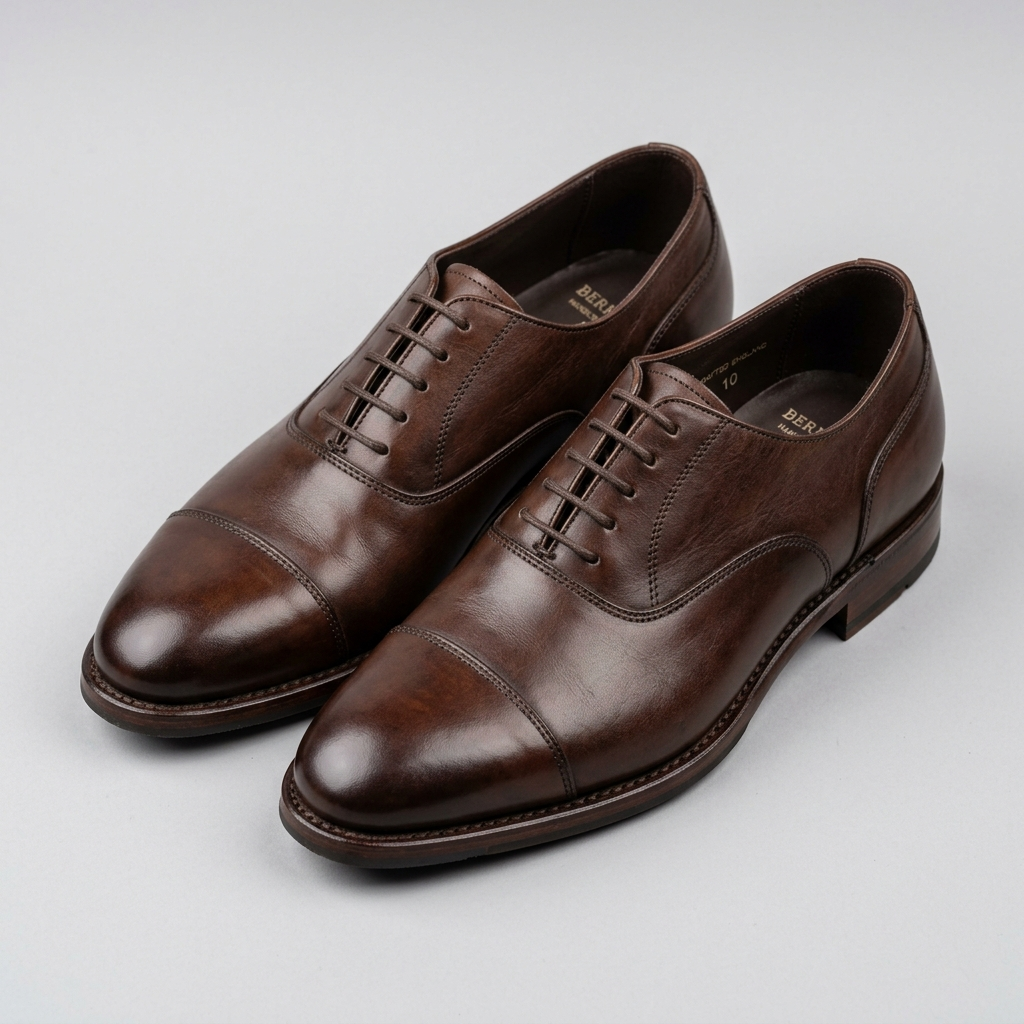
\includegraphics[width=0.9\linewidth]{vokab_300dpi/schong.png} \\
            \small\textit{De Schong (La chaussure / The shoe)}
            \vspace{0.5cm}
        }}
    \end{minipage}
    \hfill
    \begin{minipage}[t]{0.48\textwidth}
        \centering
        \textbf{Eng Suel}
        \vspace{0.5em}
        \framebox{\parbox{0.9\linewidth}{\centering
            \vspace{0.5cm}
            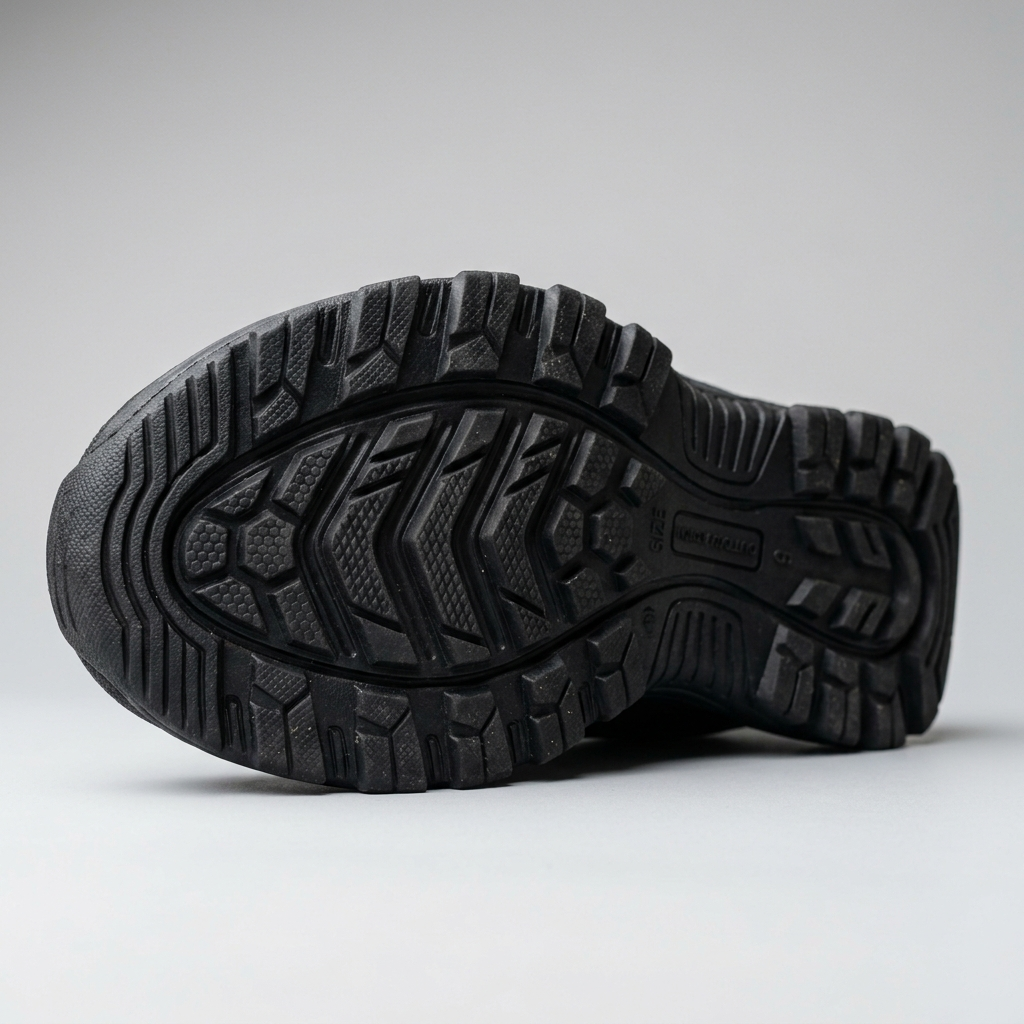
\includegraphics[width=0.9\linewidth]{vokab_300dpi/suel.png} \\
            \small\textit{D'Suel (La semelle / The sole)}
            \vspace{0.5cm}
        }}
    \end{minipage}
    
    \vspace{1.5em}
    
    \begin{minipage}[t]{0.48\textwidth}
        \centering
        \textbf{E Verkeefer}
        \vspace{0.5em}
        \framebox{\parbox{0.9\linewidth}{\centering
            \vspace{0.5cm}
            
\includegraphics[width=0.9\linewidth]{vokab_300dpi/verkeefer.png} \\
            \small\textit{De Verkeefer (Le vendeur / The assistant)}
            \vspace{0.5cm}
        }}
    \end{minipage}
    \hfill
    \begin{minipage}[t]{0.48\textwidth}
        \centering
        \textbf{Eng Rechnung}
        \vspace{0.5em}
        \framebox{\parbox{0.9\linewidth}{\centering
            \vspace{0.5cm}
            
\includegraphics[width=0.9\linewidth]{vokab_300dpi/rechnung.png} \\
            \small\textit{D'Rechnung (La facture / The receipt)}
            \vspace{0.5cm}
        }}
    \end{minipage}
    
    \vspace{1.5em}
    
    \begin{minipage}[t]{0.48\textwidth}
        \centering
        \textbf{E Schonggeschäft}
        \vspace{0.5em}
        \framebox{\parbox{0.9\linewidth}{\centering
            \vspace{0.5cm}
            
\includegraphics[width=0.9\linewidth]{vokab_300dpi/schonggeschaft.png} \\
            \small\textit{D'Schonggeschäft (Le magasin / The shop)}
            \vspace{0.5cm}
        }}
    \end{minipage}
\end{center}
